\section{Lineare Zeitinvariante Systeme (LZI)}

Für \textbf{lineare, zeitinvariante Systeme} gibt es viele Analyse- und Synthesemethoden für Regler \\
\textrightarrow\ Für \textbf{Entwurf} von Reglern gewünscht

\vspace{0.2cm}

Reale Systeme sind hingegen \textbf{nichtlinear und zeitvariant} \\
\textrightarrow\ Für \textbf{Simulation / Validierung} von Reglern gewünscht 


\subsection{Linearität (Definition)}{77}

Gegeben sei ein System 
$$ \Phi: u(t) \rightarrow y(t) \qquad y(t) = \Phi(u(t))$$
Wenn das System das \textbf{Superpositionsprinzip erfüllt}, so ist das System \textbf{linear} \\
\textrightarrow\ 'Es kommt nicht auf die Reihenfolge der Operationen an'

$$ \boxed{ \cgn{ \Phi( \alpha_A \cdot u_A(t) + \alpha_B \cdot u_B(t)) } = \cbl{ \alpha_A \cdot \Phi(u_A(t)) + \alpha_B \cdot \Phi(u_B(t)) } } $$

\begin{center}
	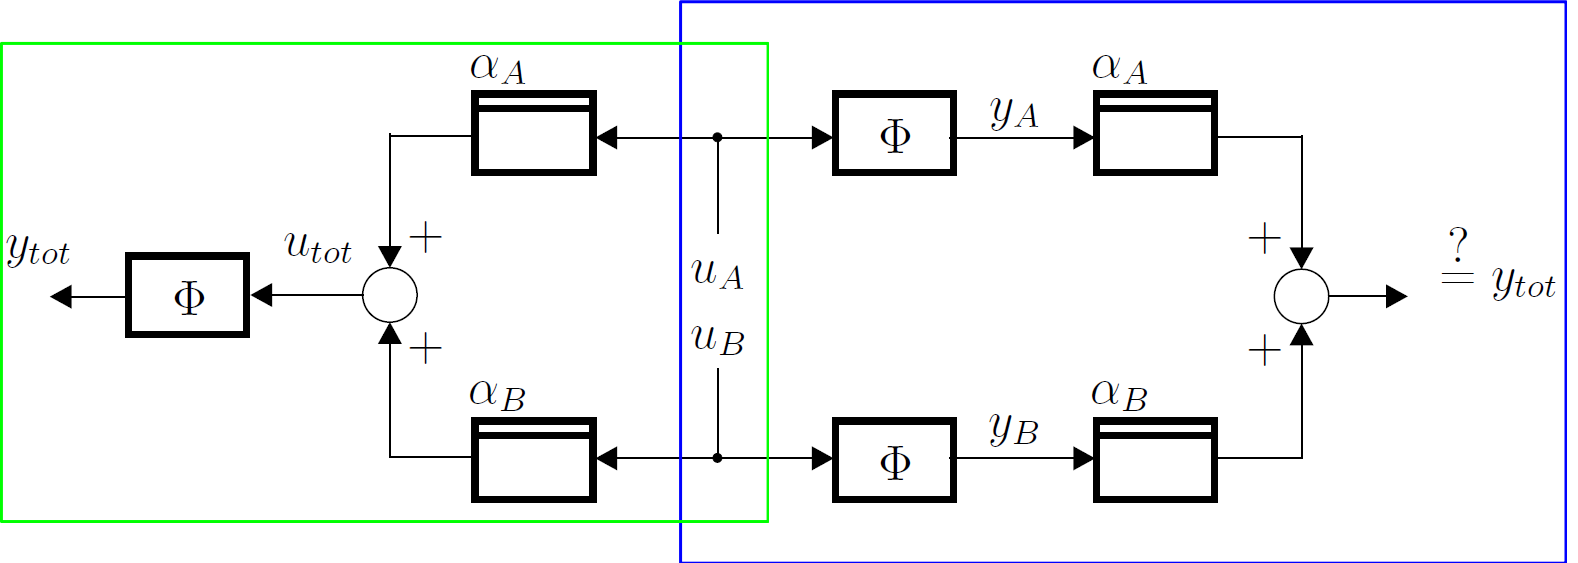
\includegraphics[width=0.9\columnwidth]{images/pruefung_linearitaet.png} 
\end{center}


\subsection{Lineare Systeme}

Alle Systeme, die mit \textbf{Differentialgleichungen mit konstanten Koeffizienten} beschrieben werden, sind linear 
$$ \boxed{ a_n y(t)^{(n)} + ... + a_1 \dot{y}(t) + a_0 y(t) = b_m u(t)^{(m)} + ... + b_1 \dot{u}(t) + b_0 u(t) } $$
\cbl{\textrightarrow\ Zeitverschiebung ändert nichts an der Linearität des Systems!}


\subsection{Zeitinvarianz (Definition)}{79}

Gegeben sei ein System 
$$\Phi: u(t) \rightarrow y(t) \qquad y(t) = \Phi(u(t))$$

Ist das System zeitinvariant, so gilt
$$ \boxed{ \Phi(u(t-T_t)) = y(t - T_t) \quad \forall \; T_t } $$
Die Antwort des Systems ist unabhängig davon, zu welchem Zeitpunkt der Eingang anliegt

\vspace{0.2cm}

\example{Wo wird $t$ ersetzt? \quad $y(t) = t \cdot u(t)$}

\begin{tabular}{ll}
	\textbf{Eingang schieben:} $t \to t - T_t$ \textbf{nur in $u$}
		& $\Phi(u(t - T_t)) = t \cdot u(t - T_t)$ \\[2pt]
	\textbf{Ausgang schieben:} $t \to t - T_t$ \textbf{in jedem $t$}
		& $y(t - T_t) = (t - T_t) \cdot u(t - T_t)$
\end{tabular}

\vspace{0.1cm}
\textrightarrow\ Eingang geschoben $\neq$ Ausgang geschoben $\Rightarrow$ \textbf{zeitvariant}


\subsubsection{Eigenschaften zeitvarianter Systeme}

\begin{itemize}
	\setlength\itemsep{5pt}

	\item Sie \textbf{können} linear sein, weil Superpositionsprinzip möglich \\
		$\Phi( \alpha_A \cdot u_A(t) + \alpha_B \cdot u_B(t), \, t)  \, = \, \alpha_A \cdot \Phi(u_A(t), \, t) + \alpha_B \cdot \Phi(u_B(t), \, t)$ \\
		$\Phi( \alpha_A \cdot u_A(t) + \alpha_B \cdot u_B(t), \, t - T_t)  \, = \, \alpha_A \cdot \Phi(u_A(t), \, t - T_t) + \alpha_B \cdot \Phi(u_B(t), \, t - T_t)$ \\
		\textrightarrow\ Nach dem Komma steht der \emph{Zeitpunkt}, zu dem das System ausgewertet wird (nicht eine Verschiebung des Eingangs): Superposition gilt zu jedem Zeitpunkt

	\item Oft ist nicht klar, ob ein Effekt zeitvariant oder nichtlinear ist
	\begin{itemize}
		\item Verschleiss in Abhängigkeit der Beanspruchung \textrightarrow\ nichtlinear
		\item Verschleiss in Abhängigkeit der Zeit (Alterung) \textrightarrow\ zeitvariant
	\end{itemize}
		

	\item Die Behandlung zeitvarianter Systeme ist manchmal einfacher als nichtlineare Systeme 
\end{itemize}


\subsection{Spickzettel: System klassifizieren}

\begingroup
\small
\renewcommand{\arraystretch}{1.25}
\begin{tabularx}{\columnwidth}{@{}lXX@{}}
	\toprule
	& \textbf{Test} & \textbf{Durchgefallen $\rightarrow$ typisch} \\
	\midrule
	\textbf{Linear?}
		& 1) Nulltest: $u \equiv 0 \Rightarrow y \equiv 0$ \newline
		  2) Superposition: $\Phi(\alpha_A u_A + \alpha_B u_B) = \alpha_A \Phi(u_A) + \alpha_B \Phi(u_B)$
		& nichtlinear: $u^2,\ |u|,\ \ln u,\ \sin u$ \newline
		  Nulltest nicht bestanden $\Rightarrow$ sicher nichtlinear; \textbf{affin} ($u + c$) nur, wenn sonst linear \\
	\textbf{Zeitinv.?}
		& $\Phi(u(t - T_t)) \overset{?}{=} y(t - T_t)$ \newline
		  (Eingang schieben $\leftrightarrow$ Ausgang schieben)
		& zeitvariant: \textbf{freies $t$} ($t \cdot u$, $\sin t$) \newline
		  DGL mit konst. Koeff. $\rightarrow$ zeitinvariant \\
	\textbf{Statisch?}
		& $y(t)$ nur von $u(t)$ (gleicher Zeitpunkt)
		& dynamisch: $\dot y,\ \ddot y,\ \int,\ u(t - T_t)$ \\
	\bottomrule
\end{tabularx}

\vspace{0.2cm}

\begin{tabularx}{\columnwidth}{@{}Xccc@{}}
	\toprule
	\textbf{System} & \textbf{linear} & \textbf{zeitinv.} & \textbf{statisch} \\
	\midrule
	$y = K \cdot u$ (Verstärkung)	& \checkmark & \checkmark & \checkmark \\
	$y = u^2$ 						& $\times$ & \checkmark & \checkmark \\
	$y = u + c$ 					& $\times$ (affin) & \checkmark & \checkmark \\
	$y = t \cdot u$ 				& \checkmark & $\times$ & \checkmark \\
	$y = \sin(t) \cdot u$ 			& \checkmark & $\times$ & \checkmark \\
	$y = u(t - T_t)$ (Totzeit)		& \checkmark & \checkmark & $\times$ \\
	$\dot y = u$ (Integrator)		& \checkmark & \checkmark & $\times$ \\
	$y = \dot u$ (Differenzierer)	& \checkmark & \checkmark & $\times$ \\
	$T \dot y + y = K u$ ($\text{PT}_1$)	& \checkmark & \checkmark & $\times$ \\
	$y = t \cdot u(t - \beta)$ 		& \checkmark & $\times$ & $\times$ \\
	\bottomrule
\end{tabularx}
\endgroup


\subsection{Umgang mit LZI-Systemen}

Wir beschäftigen uns mit LZI-Systemen, weil... 

\vspace{0.1cm}
\begin{itemize}
	\item Setzt man Systeme aus LZI Systemen zusammen, so entsteht wieder ein LZI-System 
	\item Bei seriegeschalteten LZI-Systemen kann die Reihenfolge getauscht werden
	\item Für LZI-Systeme ist ein Frequenzbereich definiert \\
 		\textrightarrow\ Sinusförmige Signale ändern Amplitude und Phase, allerdings nicht die Frequenz! \\
		\textrightarrow\ Beschreibung des LZI-Systems mittels Frequenzgang $G(\jimg \omega)$, welcher Reaktion des Systems auf eine bestimmte Frequenz beschreibt \\
\end{itemize}

Amplitudenänderung $| G(\jimg \omega) |$ ; Phasenänderung $\arg( G(\jimg \omega ))$ 


\subsection{Serieschaltung von LZI-Systemen}{82}
\label{Serieschaltung von LZI-Systemen}

\textbf{Die Reihenfolge der Blöcke darf getauscht werden}
 
\begin{center}
	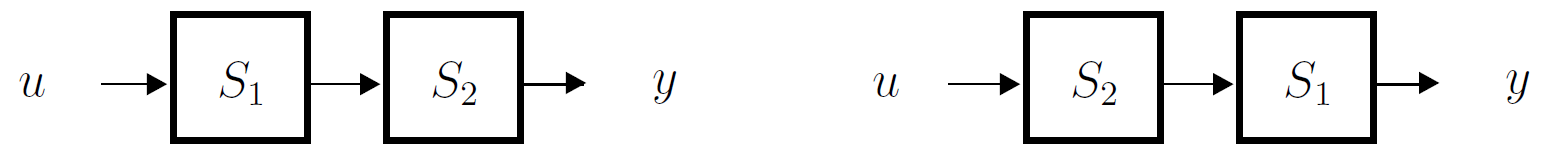
\includegraphics[width=0.85\columnwidth]{images/bloecke_tauschen.png}
\end{center}

Blöcke dürfen \textbf{verschoben werden}, müssen allerdings mit ihrer \textbf{Umkehrfunktion kompensiert werden}, um das Gesamtsystem nicht zu verändern

\begin{center}
	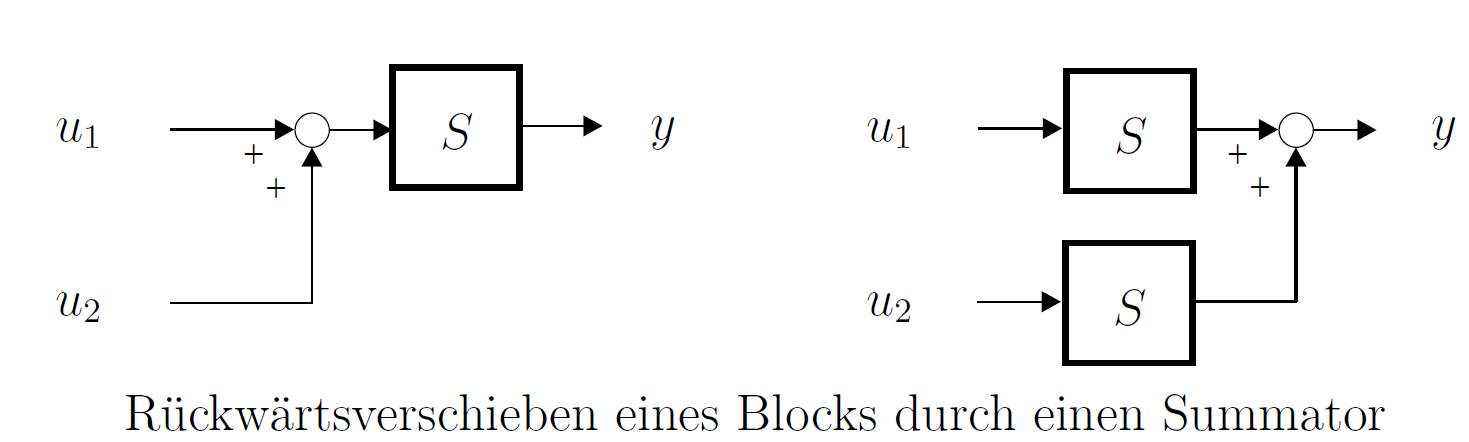
\includegraphics[width=0.73\columnwidth]{images/bloecke_schieben_1.png}
	\vspace{0.2cm}

	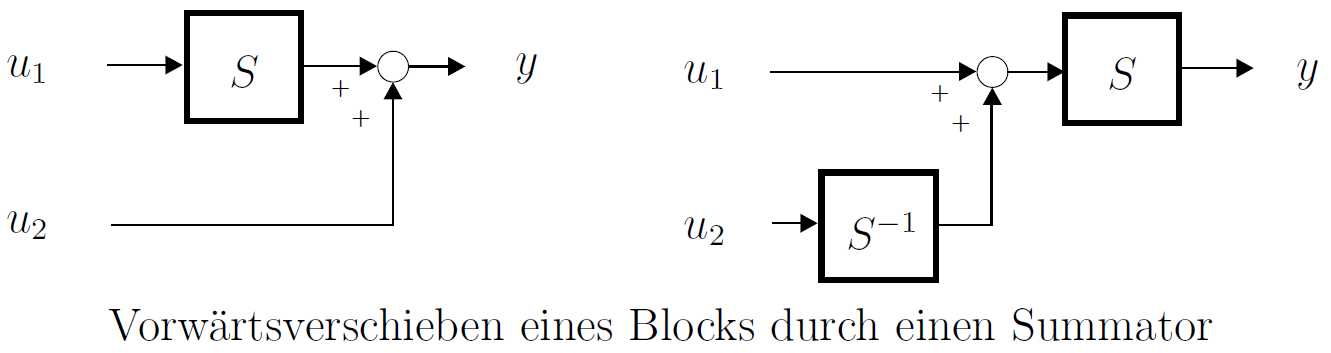
\includegraphics[width=0.73\columnwidth]{images/bloecke_schieben_2.png}
	\vspace{0.2cm}

	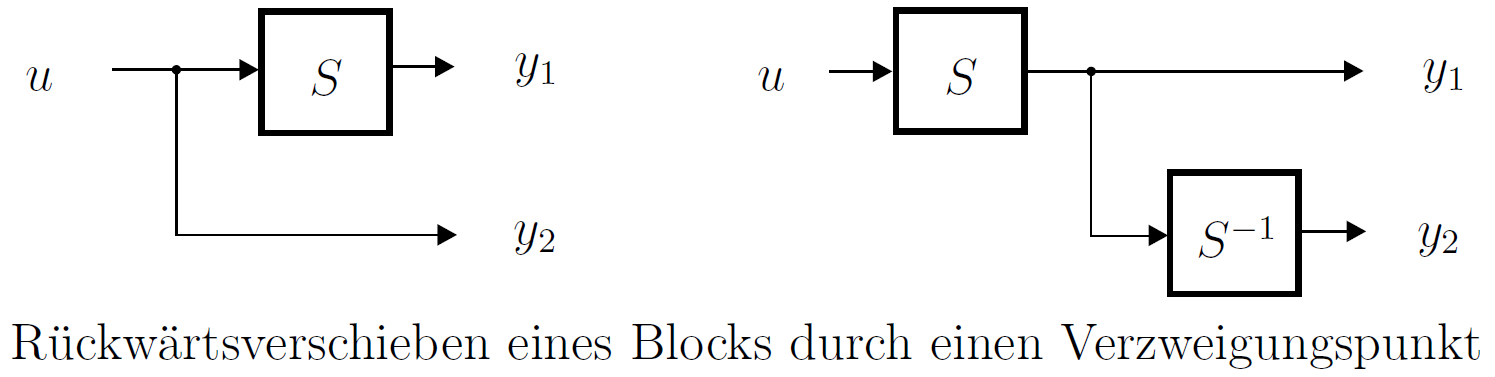
\includegraphics[width=0.73\columnwidth]{images/bloecke_schieben_3.png}
\end{center}
DGL aufstellen (Eingang des Integrators $= u - $ Rückführung, $\dot x = \dots$) und in Standardform bringen \\
\textrightarrow\ z.B. Integrator mit Rückführung 1: $\dot x + x = u$ $\Rightarrow$ $\text{PT}_1$ mit $T = 1$, $K = 1$

